\section{Ideas}
\subsection{Line search}
Line search in \ref{eqn:update_lsearch} is not working very well. 
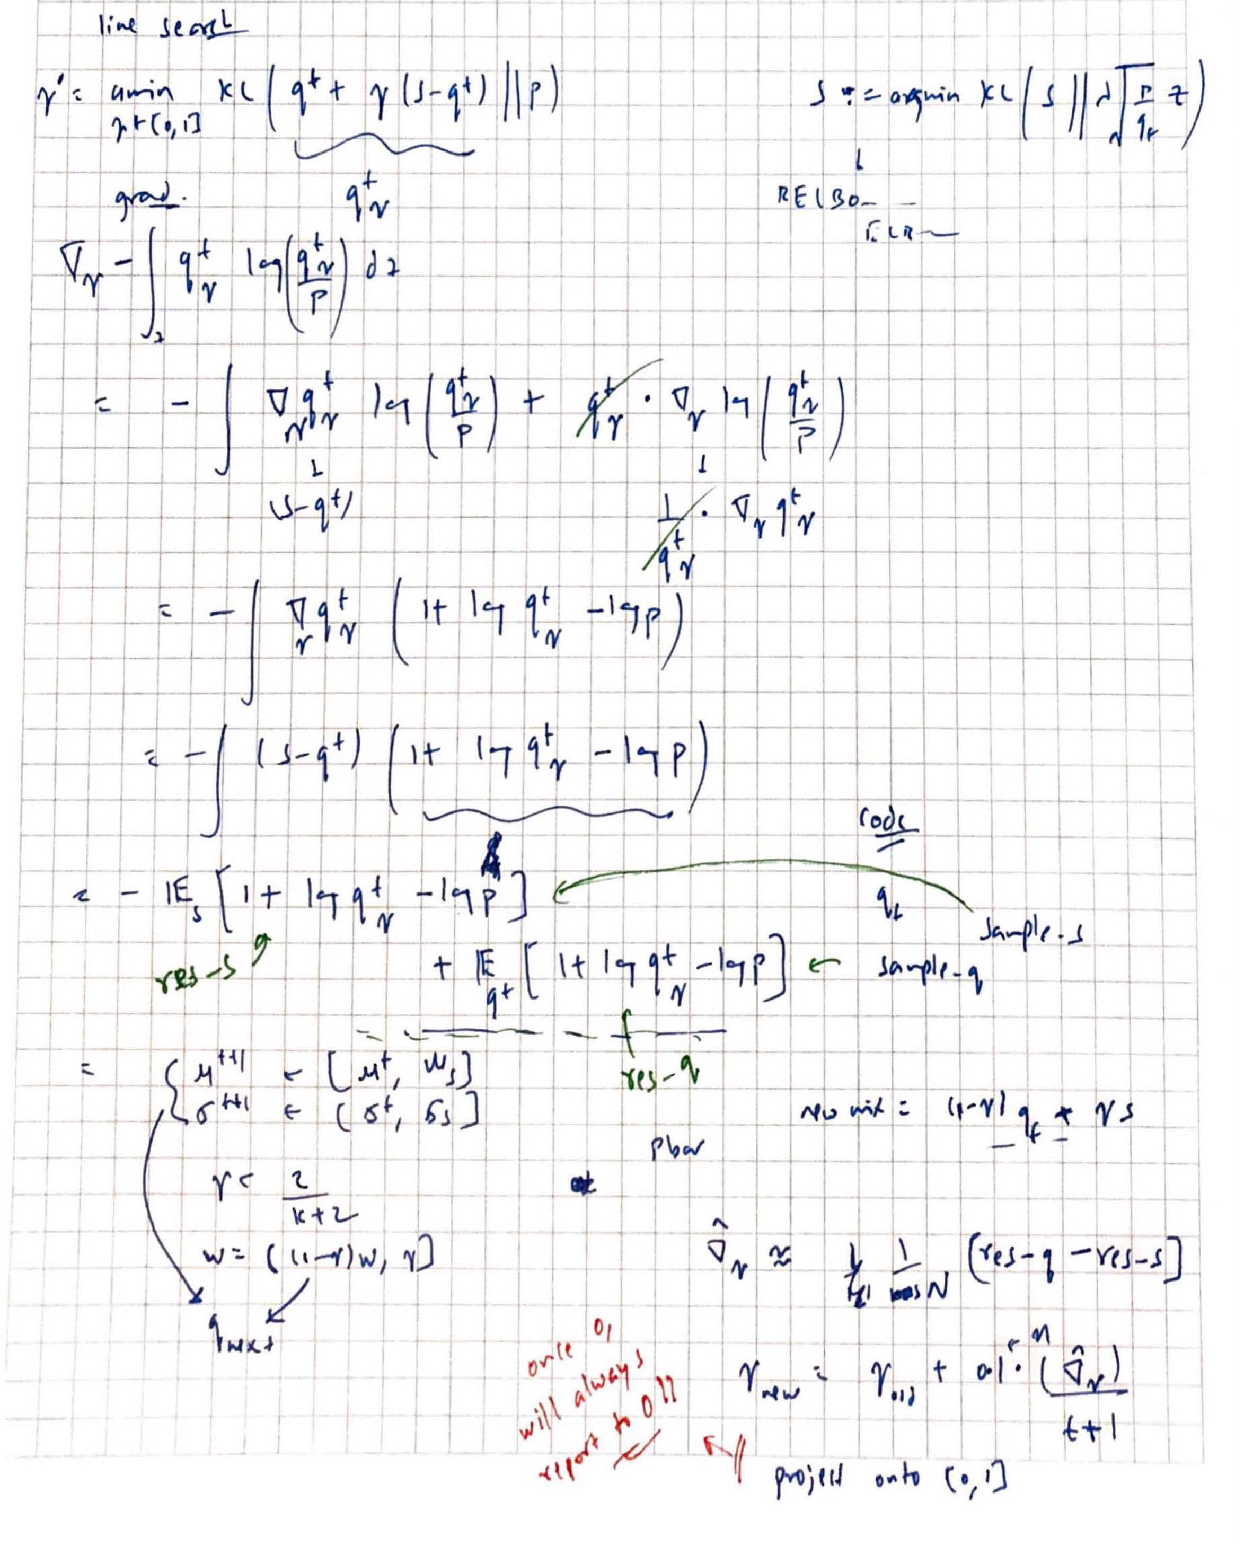
\includepdf{Thesis_notes_Nov_1.pdf}
%\inputminted[firstline=140,lastline=220,mathescape]{python}
%  {../boosting_bbvi/scripts/mixture_model_relbo.py}
\begin{minted}{python}
def line_search_dkl(weights, locs, diags, mu_s, cov_s, x, k):
  """Perform line search for the best step size gamma.
  
  Uses gradient ascent to find gamma that minimizes
  KL(q_t + gamma (s - q_t) || p)
  
  Args:
      weights: weights of mixture components of q_t
      locs: means of mixture components of q_t
      diags: deviations of mixture components of q_t
      mu_s: mean for LMO Solution s
      cov_s: cov matrix for LMO solution s
      x: target distribution p
      k: iteration number of Frank-Wolfe
  Returns:
      Computed gamma
  """
  def softmax(v):
      return np.log(1 + np.exp(v))
  # no. of samples to approximate $\nabla_{\gamma}$
  N_samples = 10
  # Create current iter $q_t$
  weights = [weights]
  qt_comps = [
      Normal(
          loc=tf.convert_to_tensor(locs[i]),
          scale=tf.convert_to_tensor(diags[i])) for i in range(len(locs))
  ]
  qt = Mixture(
      cat=Categorical(probs=tf.convert_to_tensor(weights)),
      components=qt_comps,
      sample_shape=N)
  qt = InfiniteMixtureScipy(stats.multivariate_normal)
  qt.weights = weights[0]
  qt.params = list(
      zip([[l] for l in locs], [[softmax(np.dot(d, d))] for d in diags]))
  # samples from $q_t$
  sample_q = qt.sample_n(N_samples)
  # create and sample from s
  s = stats.multivariate_normal([mu_s],
                                np.dot(np.array([cov_s]), np.array([cov_s])))
  sample_s = s.rvs(N_samples)
  # $q_{t+1}$ is mixture of $q_t$ and s with weights $(1 - \gamma)$ and $\gamma$
  # Set its corresponding parameters and weights
  new_locs = copy.copy(locs)
  new_diags = copy.copy(diags)
  new_locs.append([mu_s])
  new_diags.append([cov_s])
  # initialize $\gamma$
  gamma = 2. / (k + 2.)
  # no. steps of gradient ascent
  n_steps = 10
  prog_bar = ed.util.Progbar(n_steps)
  for it in range(n_steps):
      print("line_search iter %d, %.5f" % (it, gamma))
      new_weights = copy.copy(weights)
      new_weights[0] = [(1. - gamma) * w for w in new_weights[0]]
      new_weights[0].append(gamma)
      # create $q_{t + 1}^{\gamma}$
      q_next = InfiniteMixtureScipy(stats.multivariate_normal)
      q_next.weights = new_weights[0]
      q_next.params = list(
          zip([[l] for l in new_locs], [[np.dot(d, d)] for d in new_diags]))
      # Computes $\mathbb{E}[...] \propto \sum_{v}{\log p - \log q_{t + 1}^{\gamma}}$
      def px_qx_ratio_log_prob(v):
          Lambda = 1.
          ret = x.log_prob([v]).eval()[0] - q_next.log_prob(v)
          ret /= Lambda
          return ret
      # Samples w.r.t s
      rez_s = [
          px_qx_ratio_log_prob(sample_s[ss]) for ss in range(len(sample_s))
      ]
      # Samples w.r.t $q_{t+1}$
      rez_q = [
          px_qx_ratio_log_prob(sample_q[ss]) for ss in range(len(sample_q))
      ]
      # TODO(sauravshekhar) measure how noisy gradients are
      # Gradient ascent step, step size decreasing as $\frac{1}{it + 1}$
      gamma = gamma + 0.1 * (sum(rez_s) - sum(rez_q)) / (N_samples *
                                                          (it + 1.))
      # Projecting it back to [0, 1], too small range?
      # FIXME(sauravshekhar) if projected to 0, all iterations will be same?
      if gamma >= 1 or gamma <= 0:
          gamma = max(min(gamma, 1.), 0.)
          break
  return gamma
\end{minted}
\begin{figure}[h] \label{fig:gamma}
\centering
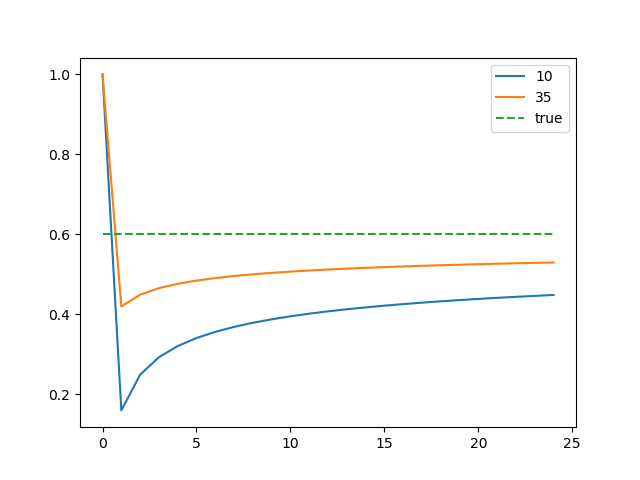
\includegraphics[width=0.9\textwidth]{plots/gamma.png}
\caption{gamma with iterations for different n\_samples}
\end{figure}
\begin{figure}[h] \label{fig:es10}
  \centering
  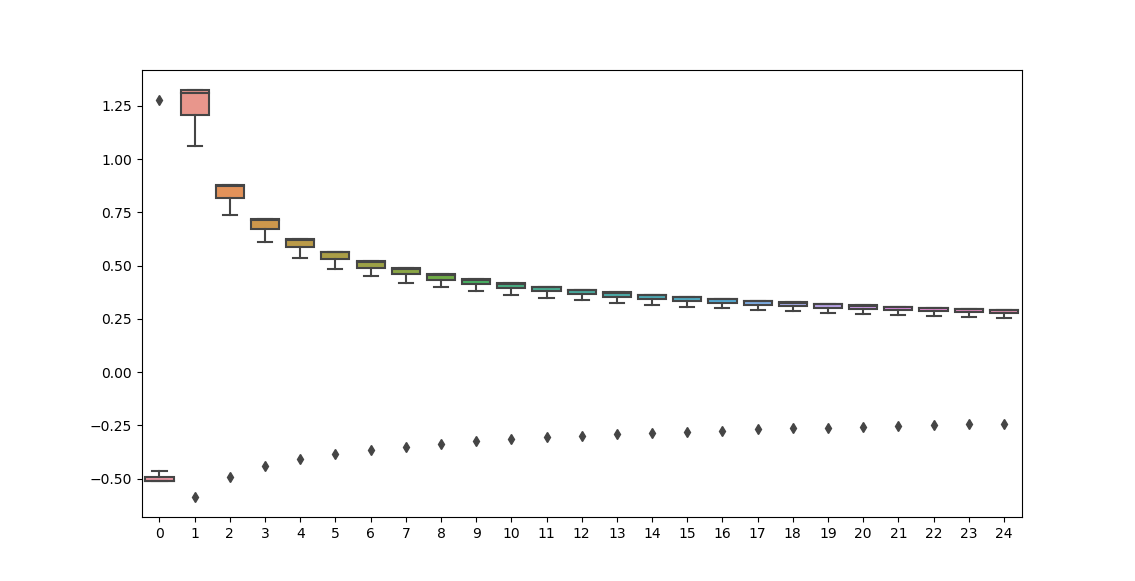
\includegraphics[width=0.9\textwidth]{plots/box_e_s_10.png}
  \caption{Boxplot for expectation w.r.t s for n\_samples = 10}
\end{figure}
\begin{figure}[h] \label{fig:es35}
\centering
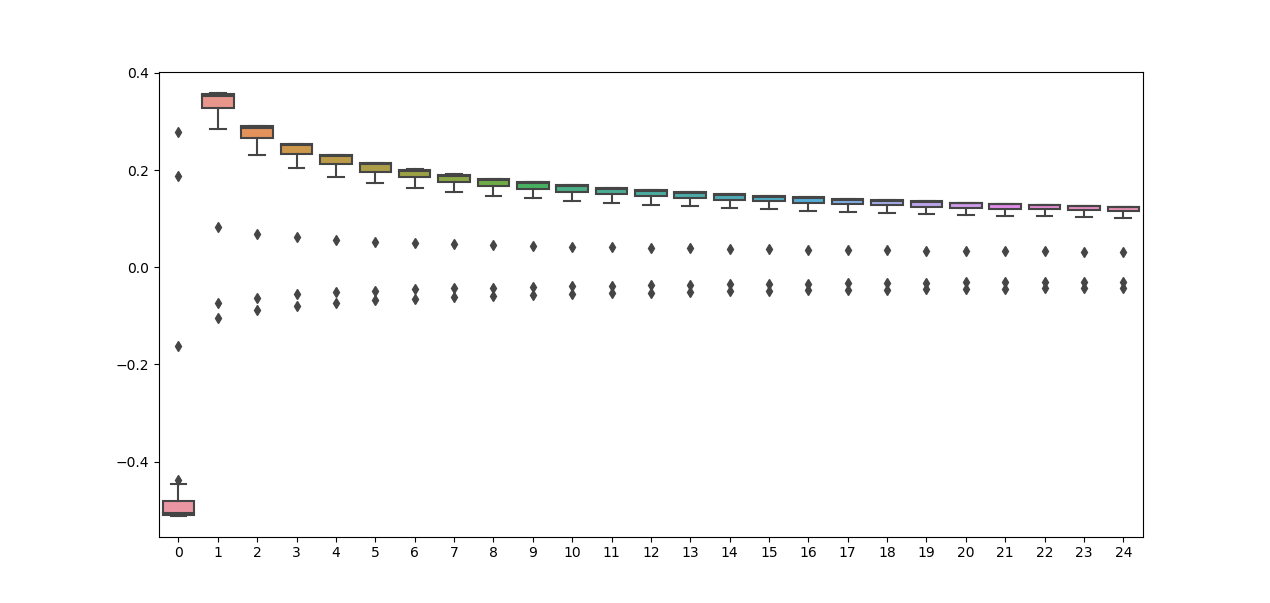
\includegraphics[width=0.9\textwidth]{plots/box_e_s_35.png}
\caption{Boxplot for expectation w.r.t s for n\_samples = 36}
\end{figure}
\TODO make $E_q$ plot with iterations starting from 1
\begin{figure}[h] \label{fig:eq10}
  \centering
  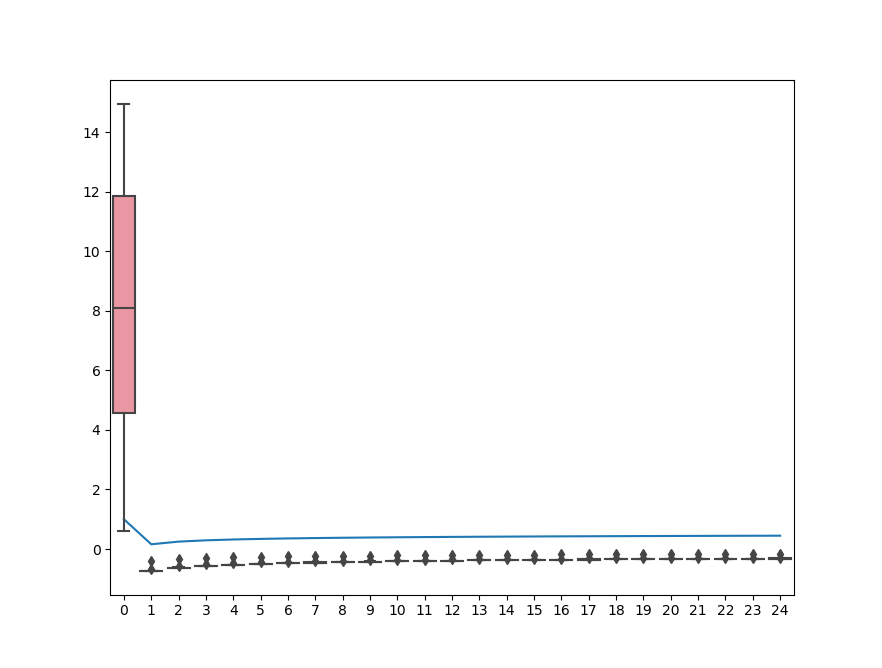
\includegraphics[width=0.9\textwidth]{plots/box_e_q_10.png}
  \caption{Boxplot for expectation w.r.t q\_t\^gamma for n\_samples = 10}
\end{figure}
\begin{figure}[h] \label{fig:eq35}
\centering
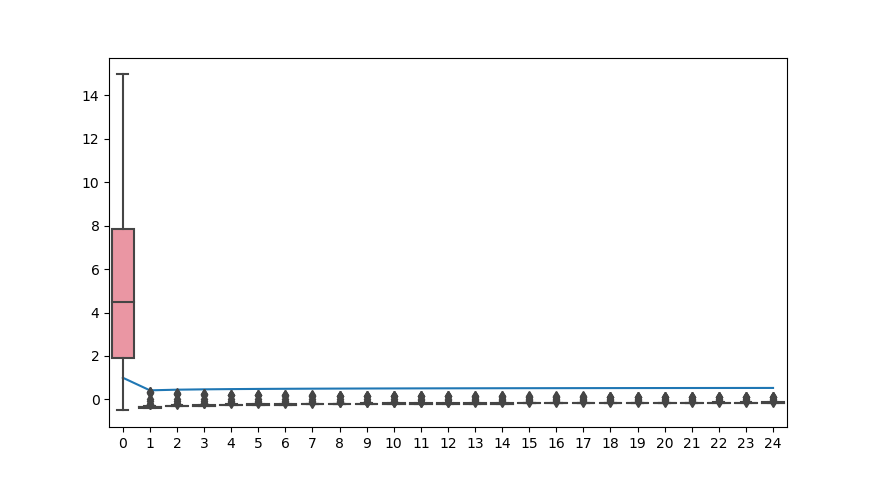
\includegraphics[width=0.9\textwidth]{plots/box_e_q_35.png}
\caption{Boxplot for expectation w.r.t q\_t\^gamma for n\_samples = 35}
\end{figure}
